\section*{Решения и комментарии}

\subsubsection*{Окружности в пространстве}% (CIRCLES IN SPACE)

Да.
Построим на $XY$-плоскости окружности радиуса $1$, центр кoторых лежит на оси $Х$ в точках $1$ по модулю $4$ (то есть точки $\dots, (-7,0)$, $(-3,0)$, $(1,0)$, $(5,0)$, $(9,0),\dots$).
Обратите внимание, что каждая сфера с центром в начале координат пересекает эти окружности ровно в двух точках.
Остаток каждой такой сферы --- это объединение окружностей.
\heart

\begin{figure}[h!]
\centering
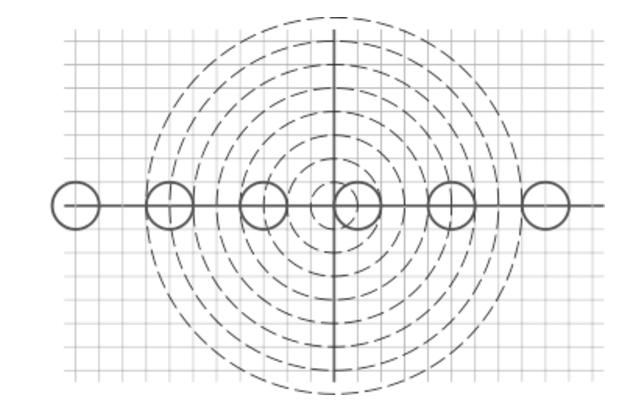
\includegraphics[scale=0.7]{Figs/Geometry/ring}
\end{figure} 

Существуют и другие способы доказательства этого факта, например, с помощью торов, но я не знаю подхода более простого и элегантного, чем приведённый выше.

Эту милую задачу на разбиения я впервые услышал от Ника Пиппенгера, %(Nick Pippenger)
профессора информатики Принстонского университета.

\subsubsection*{Магия кубов}% (MAGIC WITH CUBES)

%??? путает проекцию и сечение

Да, это можно сделать.
Для того, чтобы протащить единичный куб сквозь отверстие в другом единичном кубе, достаточно найти проекцию (второго) куба, содержащую внутри себя единичный квадрат.
Тогда во втором кубе можно проделать сквозное квадратное отверстие %(square cylindrical) 
со стороной чуть больше единицы, чтобы можно было протащить первый куб.

Можно сделать то же самое, с меньшим допуском, если второй куб только слегка меньше первого.

Самую простую (но не единственную) проекцию, которую можно использовать --- это правильный шестиугольник.
Можно увидеть этот шестиугольник, если посмотреть на куб так, что одна из вершин будет посредине.
Формально говоря, это проекция на плоскость, перпендикулярную его диагонали.

Пусть $A$ --- проекция одной из видимых граней на плоскость.
Мы видим, что её большая диагональ имеет ту же длину ($\sqrt{2}$), что и диагональ единичного куба, так как в этом направлении проекция не сокращает длину.
Если сдвинуть $A$ к центру шестиугольника и затем растянуть её до единичного куба $B$, то вытянутые углы $B$ не достанут до вершин шестиугольника (так так расстояние между противоположными вершинами шестиугольника превышает расстояние между противоположными сторонами).

\begin{figure}[h!]
\centering
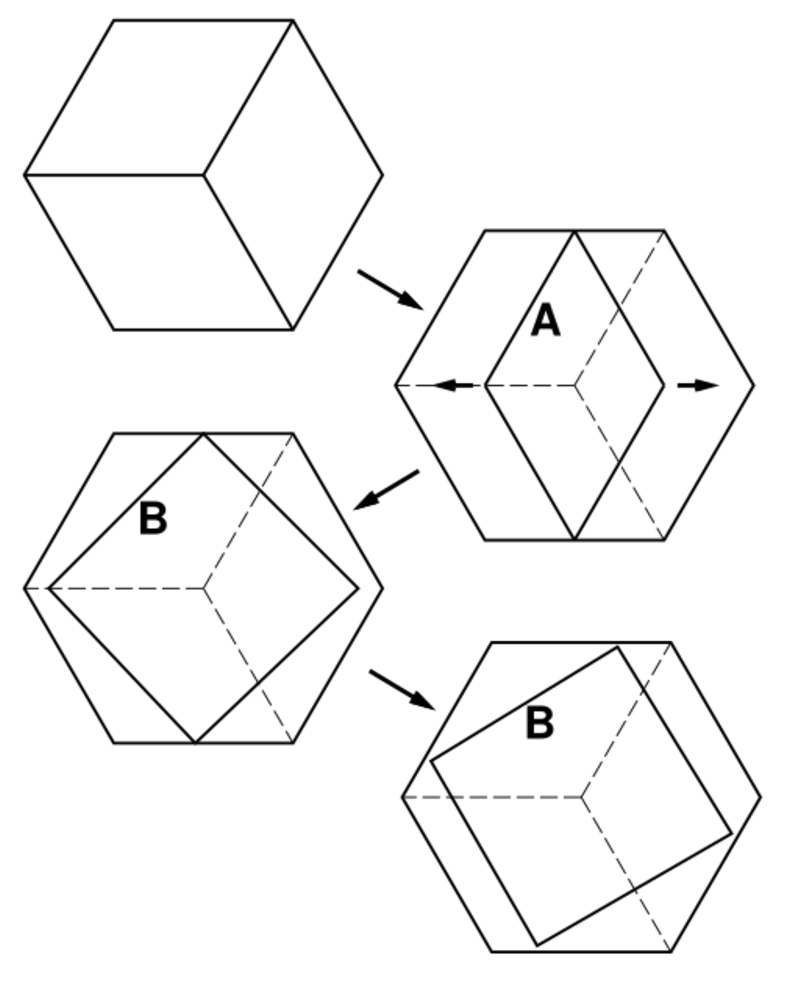
\includegraphics[scale=0.7]{Figs/Geometry/pass}
\end{figure}

Значит, если слегка повернуть квадрат $B$, то он окажется строго внутри шестиугольника.\heart

Об этой очаровательной задаче, появлявшейся в колонке Мартина Гарднера, мне напомнил Григорий Гальперин из университета Восточного Иллинойса.

\subsubsection*{Красные и синие точки}% (RED POINTS AND BLUE POINTS)

Среди всех возможных разбиений, возьмём то, при котором общая длина всех $n$ отрезков минимальна.
Мы утверждаем, что такое разбиение не будет иметь пересечений.
Действительно, если бы отрезок $uv$ пересекал отрезок $xy$, то эти отрезки были бы диагоналями выпуклого четырёхугольника $uyvx$, %???ошибка в книжке
и, по неравенству треугольника, заменив диагонали на стороны $uy$ и $xv$, мы бы уменьшили общую длину отрезков.\heart

Технику, которой мы здесь воспользовались, состоящую в нахождении нужного объекта, минимизируя или максимизируя некую величину, иногда называют вариационным методом, и он, как знают многие читатели, чрезвычайно полезен.
Следующая задача предлагает ещё один пример его применения.

Источник : Олимпиада Патнема 1960-х.

\subsubsection*{Прямая через две точки}% (LINE THROUGH TWO POINTS)

Эта знаменитая гипотеза была сформулирована Джеймсом Сильвестром в 1893 году.
Первое доказательство найдено Тибором Галлаи, %(Tibor Gallai).
но доказательство, приведённое ниже, данное в 1948 году Л. М. Келли,\footnote{L. M. Kelly American Mathematical Monthly, Vol.55} 
часто упоминалось Палoм Эрдёшем, как пример доказательства из «Книги».

\begin{figure}[h!]
\centering
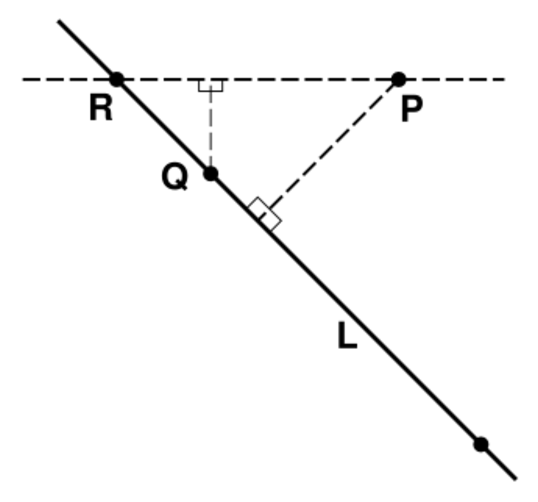
\includegraphics[scale=0.7]{Figs/Geometry/kelly}
\end{figure}

Предположим, что каждая прямая, проходящая через две точки множества $X$, содержит, по меньшей мере, три точки из $X$.
Идея состоит в том, чтобы рассмотреть прямую $L$ и точку $P$, не лежащую на $L$, такие что расстояние от $P$ до $L$ минимально.

Поскольку $L$ содержит, по меньшей мере, три точки из $X$, две из них, скажем, $Q$ и $R$, лежат с одной стороны от перпендикуляра, опущенного из точки $P$ на прямую $L$.
Но тогда, если $R$ --- дальняя точка, то $Q$ находится ближе к прямой $PR$, чем $P$ к $L$ --- противоречие.\heart

\subsubsection*{Пары на максимальном расстоянии}% (PAIRS AT MAXIMUM DISTANCE)

Для решения данной задачи из олимпиады Патнема 1957 года, будет полезно следующее наблюдение: если $A,B$ и $C,D$ --- две «максимальные пары» (то есть пары точек из $X$, расстояние между которыми равно $d$), тогда отрезки $AB$ и $CD$ пересекаются (иначе одна из диагоналей прямоугольника $ABCD$ будет иметь длину, превышающую $d$).

Предположим, что утверждение задачи неверно, и пусть наименьший контрпример имеет размер $n$.
Поскольку максимальных пар больше, чем $n$, и каждая состоит из двух точек, то должна существовать такая точка $P$, которая принадлежит трём максимальным парам (пусть это будут пары с точками $A$, $B$, $C$).
Каждые два из отрезков $PA$, $PB$ и $PC$ должны в точке $P$ образовывать угол максимум в 60\degree.
Один из этих отрезков, скажем, $PB$, %???ошибка в книжке
должен лежать между двумя другими.

Но тогда точке $B$ будет довольно сложно образовать максимальную пару с какой-либо другой точкой, так как, если $BQ$ была бы максимальной парой, то отрезок $BQ$ должен бы был пересекать и $PA$, и $PC$, что невозможно.
Значит, можно выбросить $B$ из множества $X$, теряя при этом только одну максимальную пару и получая таким образом меньший контрпример.
Это противоречие завершает доказательство.\heart

\subsubsection*{Монах на горе}% (MONK ON A MOUNTAIN)

Пожалуй, самое лёгкое решение --- это представить себе, что у монаха есть близнец, которому даны указания взобраться на гору во вторник утром точно тем же путём, каким шёл монах в понедельник.
Тогда монах должен встретить близнеца по дороге вниз, или, если они идут разными тропами, оказаться в какой-то момент на одной с ним высоте.\heart

(Возможно, эта задача показалась вам слишком лёгкой, не волнуйтесь, гораздо более сложная её версия ожидает вас в Главе 11 --- «Крепкие орешки»)

На эту древнюю задачу можно смотреть как на пример применения теоремы о промежуточном значении --- очень полезной теоремы утверждающей, что непрерывная функция обязана принять все свои промежуточные значения.
В нашем случае функцией можно выбрать разность между высотой, на которой оказался монах в определённое время дня в понедельник, и высотой, на которой он был в то же самое время дня во вторник.
Начальное значение функции будет отрицательным (примерно минус высота горы Фудзияма), а конечное значение --- положительным, таким образом, в некой точке функция должна обратиться в ноль.

Можно считать, что высота, на которой находился монах в каждый из дней, представлена графиком, и два графика наложены друг на друга.
Тогда должна существовать точка (или точки), где они пересекаются.

Другими  известными примерами применения теоремы о промежуточном значении являются задачи о том, можно ли вписать озеро Мичиган в квадрат, и можно ли  разрезать сэндвич (плоскостью) так, чтобы разделить ветчину, сыр и хлеб точно пополам.

\subsubsection*{Раскраска многогранника}% (PAINTING THE POLYHEDRON)

Предположим, что сфера вписана в $P$, триангулируем грани $P$, используя точки касания сферы.
Тогда треугольники по обе стороны любого ребра конгруэнтны, и, значит, имеют одинаковую площадь.
В каждой такой паре не более одного красного треугольника.
Из этого следует, что площадь красных граней не превосходит площади зелёных, что противоречит условию задачи.\heart

\begin{figure}[h!]
\centering
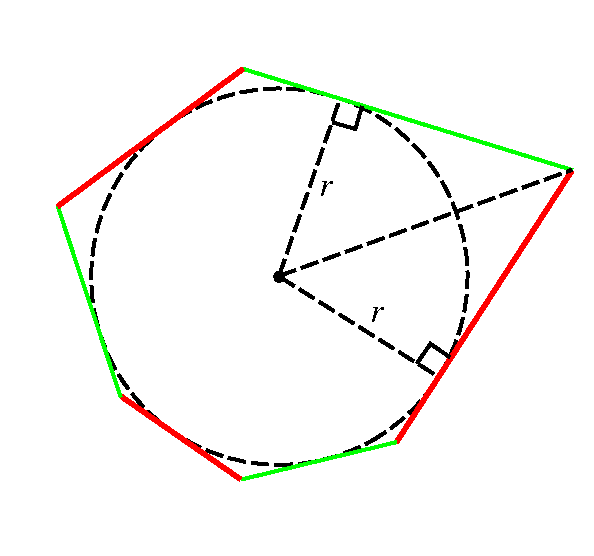
\includegraphics[scale=0.5]{Figs/Geometry/polygon}
\end{figure}%???цвет

Эта задача пришла ко мне от Эмины Солянин %(Emina Soljanin) 
из лабораторий Белла.
На иллюстрации представлена двумерная версия, где стороны и вершины многоугольника заменяют грани и рёбра многогранника $P$.

\subsubsection*{Круглые тени}% (CIRCULAR SHADOWS)

Эта, способная вас смутить, задача, пришла к нам из 5-й Всесоюзной Математической Олимпиады в Риге 1971 года.
Простой способ превратить ваше интуитивное решение в строгое доказательство состоит в следующем: --- поместим тело между двумя плоскостями, перпендикулярными одновременно обеим плоскостям проекций, и начнём их сдвигать.
В  момент, когда они коснутся тела, они пройдут через противолежащие точки каждой из проекций, и расстояние между параллельными плоскостями будет равно общему диаметру проекций.
\heart

\subsubsection*{Полоски на плоскости}% (STRIPS IN THE PLANE) 

Как и предыдущая, данная задача, версия которой появлялась в ранних олимпиадах Патнема, представляет собой ещё один пример «интуитивно очевидного» факта, который всё-таки нужно доказать.

\medskip

Поскольку сложно сравнивать бесконечные величины, имеет смысл сосредоточиться на какой-нибудь конечной части плоскости.
Мы не можем контролировать углы между полосками, так что логично будет рассмотреть круг $D$ радиуса $r$.

Предположим, полоски имеют ширину $w_1$, $w_2,\dots$, которые в сумме дают $1$.
Оказывается, что они не могут покрыть даже круг $D$, при $r=1$.
Действительно, пересечение $D$ с полоской шириной $w$ лежит в прямоугольнике шириной $w$ и длиной $2$, и, следовательно, его площадь меньше $2w$.
Таким образом, площадь, покрытaя полосками внутри $D$, меньше $2$, а площадь $D$, конечно же, $\pi>2$.
\heart 

Доказательство выше говорит, что чтобы покрыть единичный круг, суммарная ширина полосок должна быть больше $\pi/2$, но на самом деле, это можно сделать, только если суммарная ширина хотя бы 2 (в этом случае параллельные полоски дают решение).
Есть очень милое доказательство этого утверждения:
идея в том, чтобы продолжить задачу в 3-мерное пространство, взяв за $D$ сечение единичного шара, проходящее через его центр.
Предположим, круг покрыт полосками, суммарная ширина которых $W$, и пусть $S$ --- одна из полосок шириной, скажем, $w$.
Можно предположить, что либо оба края полоски пересекают $D$, либо один край пересекает и один касается.
Проектируя $S$ вверх и вниз на поверхность шара, мы получаем пояс (или шапочку),
окружающую шар --- чья площадь, здесь вы можете продемонстрировать своё знание анализа, равна 
$2\pi w$, независимо от положения полоски!

Поскольку площадь поверхности шара равна $4\pi$, чтобы её покрыть потребуется $W\ge 2$,
а если не покрыта поверхность шара, то и круг не покрыт.

\subsubsection*{Ромбики в шестиугольнике}% (DIAMONDS IN HEXAGON)

\begin{figure}[h!]
\centering
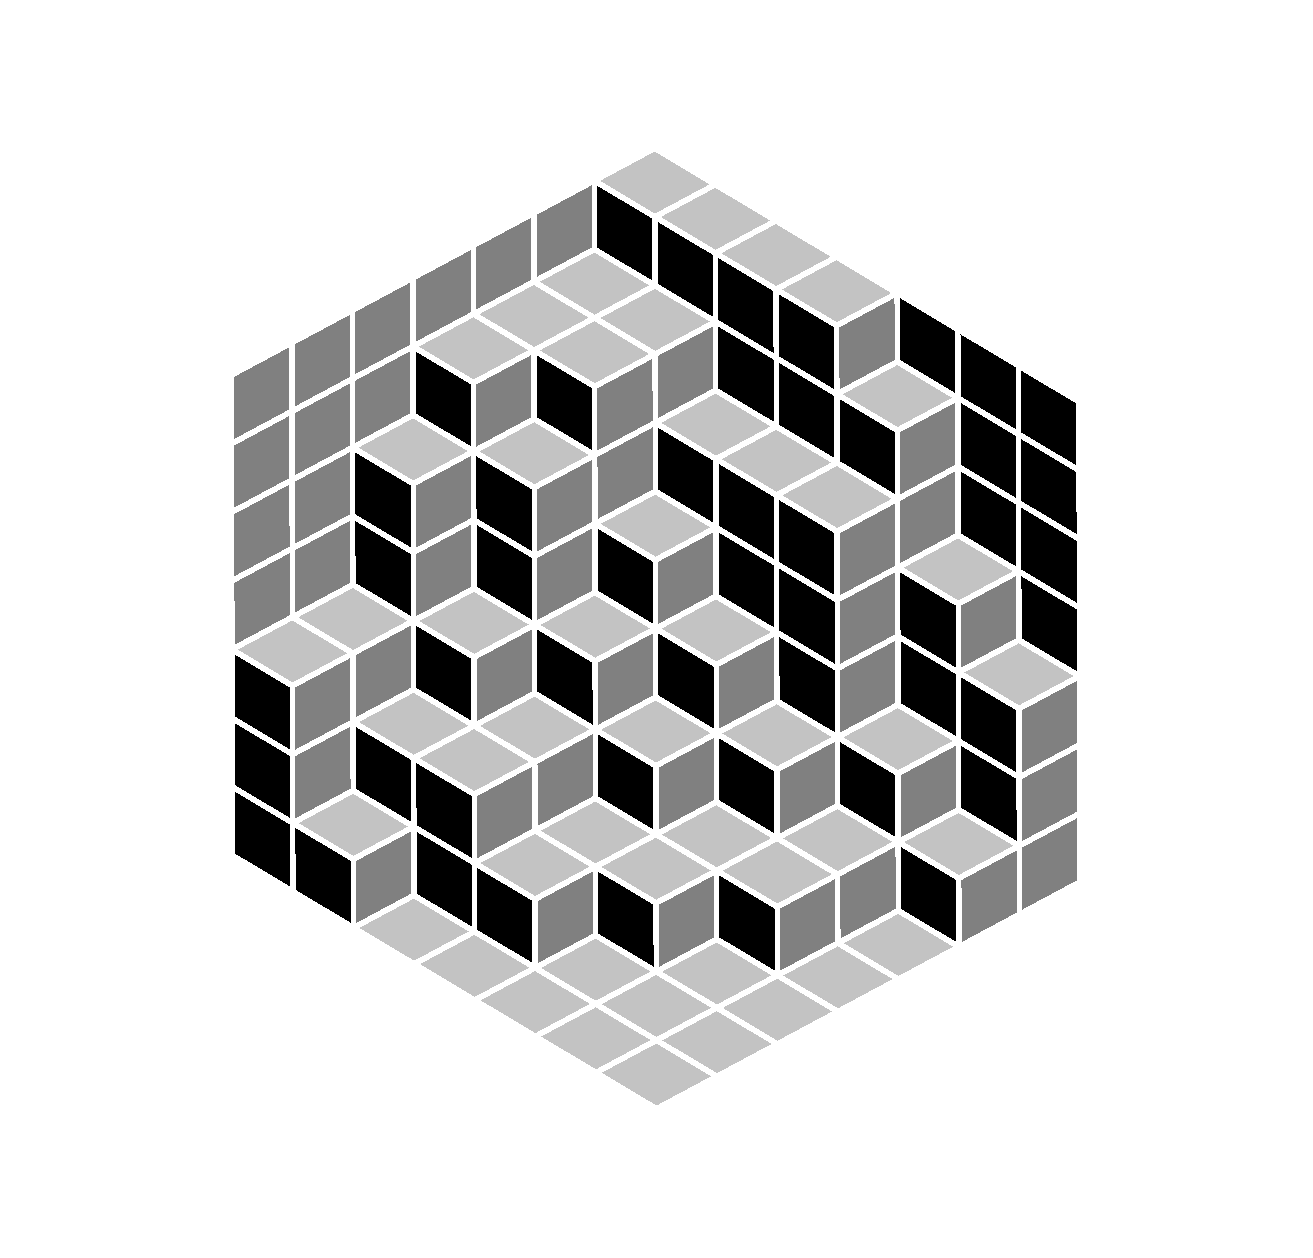
\includegraphics[scale=0.5]{Figs/Geometry/diamonds}
\end{figure}
\heart

Доказательства без слов стали очень популярной темой в журналах «Mathematics Magazine» и «The College Mathematics Journal» Математической aссоциации Америки.
Вы также можете найти эти задачи в книгах Роджера Б. Нелсена.%
\footnote{Proofs Without Words and Proofs Without Words II, by Roger B Nelsen, MAA.}
Задача о «ромбиках» в шестиугольнике появляется в его первой книге как «Задача o калиссонах»\footnote{The Problem of the Calissons}.

\subsubsection*{Замощение ромба}% (RHOMBUS TILING)

Пусть $u$ --- одна из сторон $2n$-угольника.
Назовём $u$-ромбом любой из $n-1$ ромбов, у которых $u$ параллельна одной из сторон.
В нашем замощении плитка, прилегающая к $u$-стороне, должна быть $u$-ромбом, как и плитка с другой стороны от этого ромба, и так далее, пока мы не достигнем противоположной стороны $2n$-угольника.
Заметьте, что каждый шаг на этом пути делается в одном направлении (а именно, вправо или влево) относительно вектора $u$. 
Также должен вести себя и любой другой путь, содержащий $u$-ромб.
Но тогда не может быть других $u$-ромбов, поскольку они образовали бы дополнительный путь, которому негде было бы закончиться.

\begin{figure}[h!]
\centering
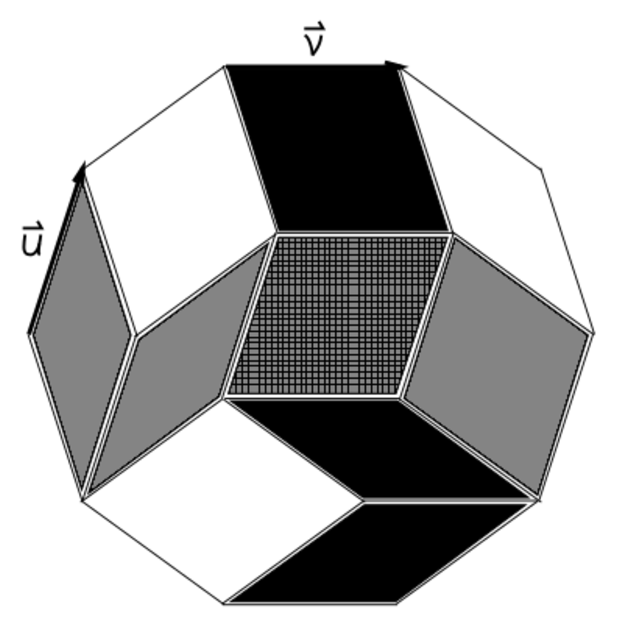
\includegraphics[scale=0.5]{Figs/Geometry/dimers}
\end{figure}

Аналогично определяемый путь для другой стороны $v$ должен пересечь $u$, и их общая плитка, разумеется, образована сторонами $u$ и $v$.
Могут ли они пересечься дважды?
Нет, поскольку при повторном пересечении внутренний угол ромба между $u$ и $v$ превысил бы $\pi$.\heart

Данная задача досталась мне от Дейны Рэндaлл из Технологическoго института Джорджии.
%(Dana Randall of Georgia Tech).

\subsubsection*{Векторы на многограннике}% (VECTORS ON A POLYHEDRON)

На эту задачу обратил моё внимание Ювал Перес, профессор факультета статистистики Калифорнийского университета в Беркли. %( (Yuval Peres of the Department of Statistics at UC Berkeley).
Самый простой способ понять, что сумма векторов должна быть нулевой --- это провести следующий умственный эксперимент.
Накачаем воздух в (жёсткий) многогранник и отметим, что давление на грань есть сила, действующая по нормали, и её величина пропорциональна площади поверхности грани.
Давление на грани должно быть уравновешено, иначе многогранник бы двигался по собственному усмотрению.
\heart

\subsubsection*{Три окружности}% (THREE CIRCLES)

Эта задача является лучшим известным мне примером эффективности повышения размерности пространства.
Заменим каждую окружность сферой с центром на плоскости, чьё пересечение с плоскостью и есть заданная окружность.
Теперь, каждой паре сфер соответствует конус, и искомые точки являются вершинами трёх конусов. %???забыл про центр

Но все эти вершины лежат на плоскости, которая касается сфер сверху, и точно так
же, они все лежат на плоскости, которая касается сфер снизу.
Значит, oни принадлежат пересечению двух плоскостей --- прямой! \heart

Похоже, что это старинная классическая задача.
Впервые я услышал её от Дейны Рэндaлл, %(Dana Randall), 
из колледжа компьютерных наук Технологическoго института Джорджии.
Вадим Жарницкий, из университета Иллинойса, заметил, что можно задать аналогичный вопрос о четырёх сферах в 3-мерном пространстве: будут ли вершины шести конусов, определяемых данными сферами, лежать на одной плоскости?
Так оно и будет, и один из способов это доказать --- повысить размерность до 4-х.

\subsubsection*{Сфера и четырёхугольник}% (SPHERE AND QUADRIATERAL)

Эту задачу я получил от Тани Ховановой, приглашенного научного сотрудника Принстонского университета в рамках программы по прикладной и вычислительной математике.
У неё есть коллекция задач, которые она зовёт «гробами».
Oна пишет:

\medskip

\begin{trivlist}\leftskip=1cm\rightskip=.5cm
\item\relax«Математико-механический факультет Московского Государственного университета, самая престижная математическая школа России, в своё время (1975) очень активно пытался препятствовать поступлению еврейских (и других „нежелательных“) студентов на факультет.
Один из методов, используемых в этих целях, был таков: неугодным студентам давался на устном экзамене отдельный набор задач.
Задачи эти выбирались очень аккуратно, они имели простое решение (дабы факультет мог избежать скандала), которое было почти невозможно найти.
Любому, кто не решал задачу, могли с лёгкостью отказать в приёме, так что подобная система эффективно контролировала поступление на МехМат.
Такого сорта задачи неформально называли \glqq гробами\grqq.» %???
\end{trivlist}

\medskip

Следующее решение, действительно, найти трудно, но, полагаю, не совсем невозможно.
Сначала следует понять, что для того, чтобы пространственный четырёхугольник оказался плоским достаточно, чтобы его диагонали (или их продолжения) пересекались в некоторой точке.
Заметим, что каждая вершина четырёхугольника $i$ находится на одинаковом расстоянии $d_i$ до точек касания образующих её сторон.
Снабдим вершину $i$ массой $1/d_i$, тогда центр масс двух соседних вершин есть точка касания их общей стороны.
Из этого следует, что центр масс всех четырёх точек лежит на отрезке, соединяющем противоположные точки касания --- это и есть искомая точка.
\heart

\subsubsection*{Восьмёрки на плоскости}% (FIGURES 8S IN THE PLANE)

Эта задача известна уже около 50-ти лет.
Мне говорили, что автором её является великий тополог, профессор университета штата Техас Роберт Ли Мур (1882---1974). %(Robert Lee Moore; 1882—1974).
Читатели, незнакомые с разными степенями «бесконечности», могут уже пребывать в недоумении: ведь очевидно, что на плоскости можно нарисовать бесконечно много восьмёрок, например, поместив по одной восьмёрке внутри каждой клетки квадратной решётки.
О таком множестве мы говорим, что оно счётно. 
Это означает, что восьмёрки можно пронумеровать натуральными числами, так, что каждой восьмёрке будет соответствовать только одно число.

Множество целых чисел, множество всех пар целых чисел, и, таким образом, множество рациональных чисел --- всё это счётные множества, но, как было замечено блестящим (но зачастую депрессивным) математиком Георгом Кантором в 1878 году, множество вещественных чисел не является счётным.
Можно было бы начертить на плоскости концетрические окружности всех возможных положительных вещественных диаметров, и, следовательно, если бы в задаче говорилось об окружностях вместо восьмёрок, ответ был бы «несчётное число», или, более точно, «равномощно множеству вещественных чисел».% (the cardinality of the reals).

Тем не менее, можно нарисовать только счётное число восьмёрок.
Каждой восьмёрке поставим в соответствие пару рациональных точек (точки на плоскости, чьи обе координаты --- рациональные числа), по одной в каждой петле.
Никакие две восьмёрки не могут иметь общих пар точек.
Значит, мощность множества восьмёрок не превышает мощности множества пар из пар рациональных чисел, которое является счётным.\heart

Более хитрую версию данной задачи смотрите в Главе 11 («Крепкие орешки»).
